% tex for data

\documentclass{article}
\usepackage{url,graphicx,tabularx,array,amsmath,amssymb,amsthm,booktabs,float}
\usepackage[margin=.65in]{geometry}
\graphicspath{{C:/Users/Colin/Documents/GitHub/533-proj/}{C:\Users}}
\begin{document}
\noindent \textit{Data:}\\\\
The data analyzed is hard drive testing data from the company, Backblaze.  Since 2013, Backblaze has been continuously spinning hard drives in controlled storage pods.  Hard drives are run till they fail or are right censored.  When a hard drive fails it is permanently removed from testing.  In addition, new hard drives are regularly added to the testing sample.  The latest data provided by Backblaze goes from January 1, 2015 to September 30, 2015.  Blackblaze provides over 70 variables on each hard drive; we wll focus on the following subset: an indicator variable for the last day the hard drive was in service before failing, the number of hours a hard drive has been on test, and the model/brand of each hard drive.\\\\
The raw data download from Backblaze contained 54,398 unique drives.  Before analyzing the data, however, we removed certain observations.  Any models with fewer than 100 drives in testing were excluded.  Also, drives that failed in fewer than 20 days were removed.  There were some other bizarre observations in the data; for example, hard drives listed as being in test for over 10 years or drives that entered and exited the sample on the same day.  These bizarre observations were likely due to mis-coding and were dropped.  After cleaning the data we had a sample size of 52,811 total drives for analysis.\\\\
The final sample included 21 hard drive models.  Below is a summary of the distribution of failures, and total testing time for each model.  The total number of failures was 1030.  The majority of those failures came from models 5, 7, 9, and 11.  Not surprising, model 11, which had the most failures also had the longest total testing time; however, this relationship was not uniform across models.  Model 1 had the 2nd longest total testing time, but relatively few failures.
\begin{figure}[H]
\centering
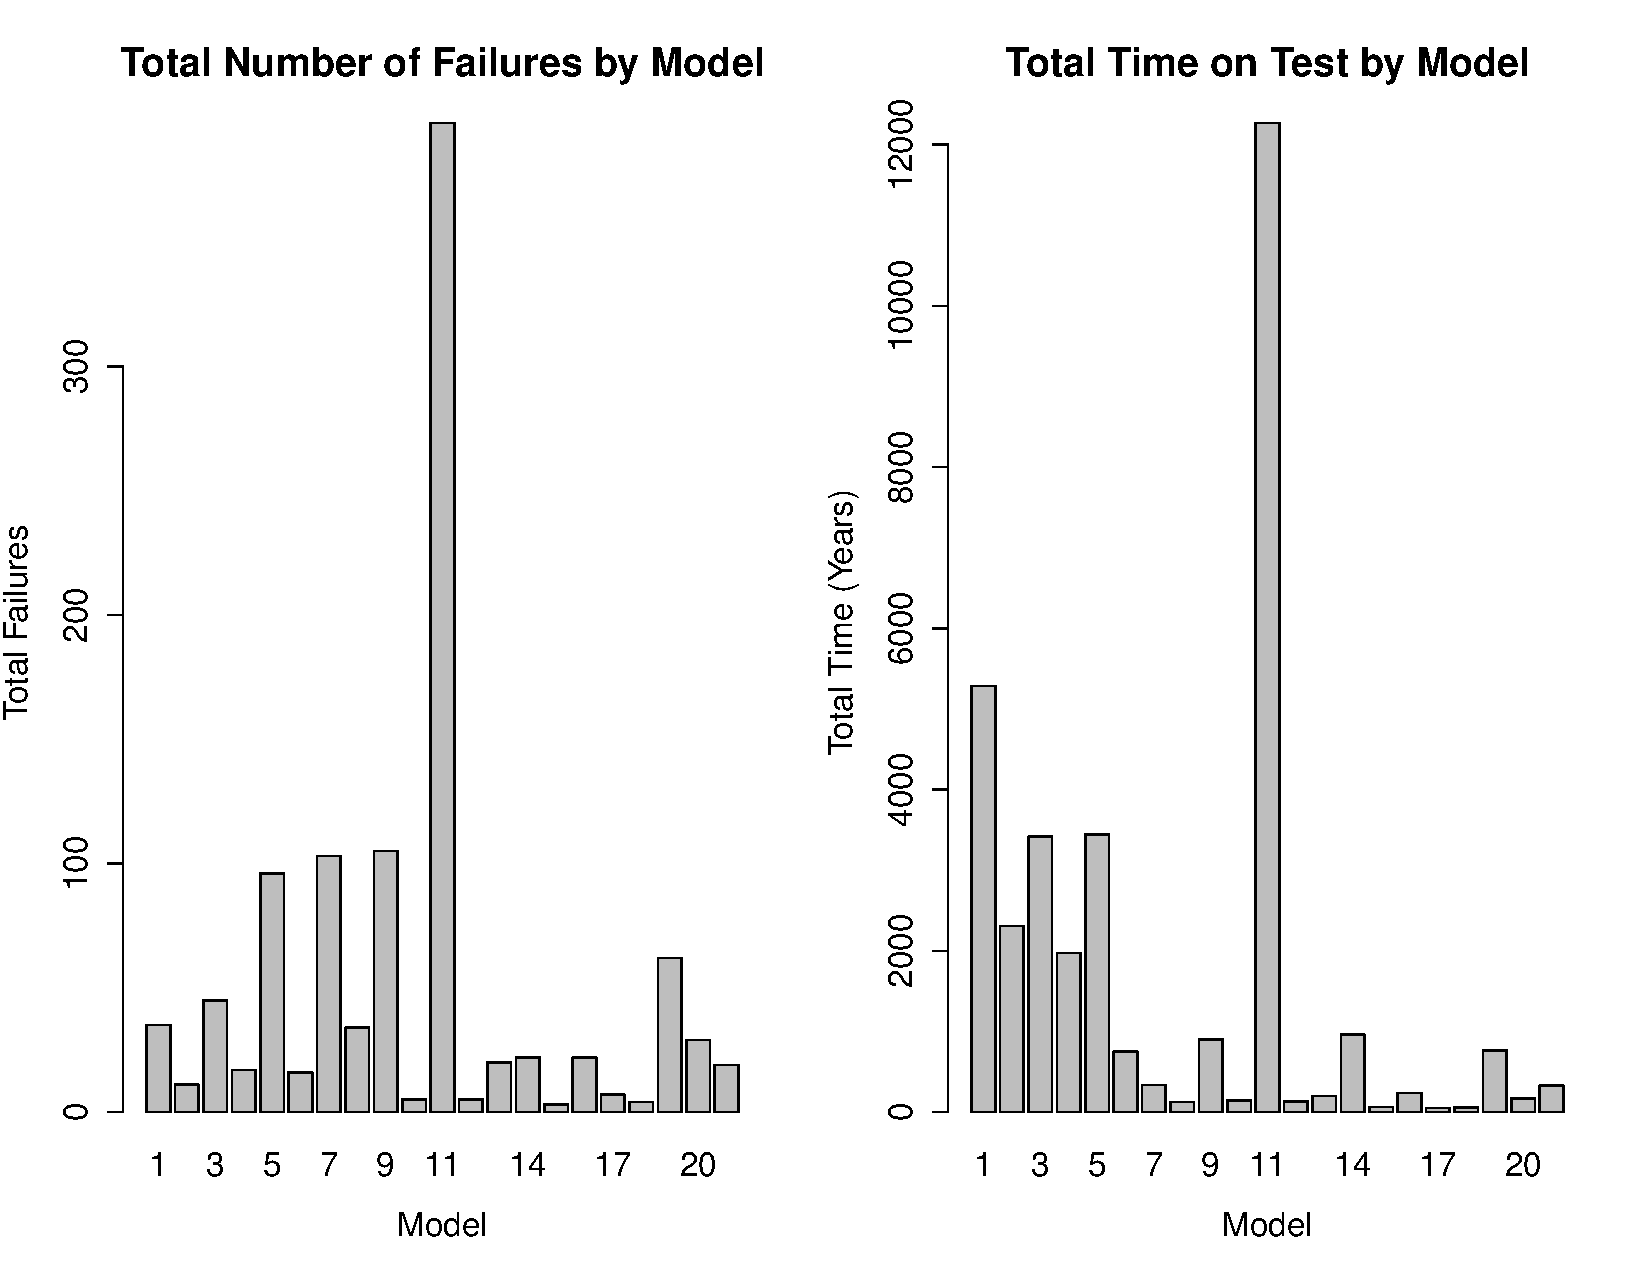
\includegraphics[height=12cm]{sumstat1.pdf}
\end{figure}
\noindent We also examined the distribution of failure times.  The shape is slightly skewed to the right with the majority of failures occurring within 250 days. But this distribution is not consistent across models. As exemplified when looking at just model 11, the failure times vary depending on the brand of the hard drive.  This provides further evidence that a separate model should be fit for each brand.
\begin{figure}[H]
\centering
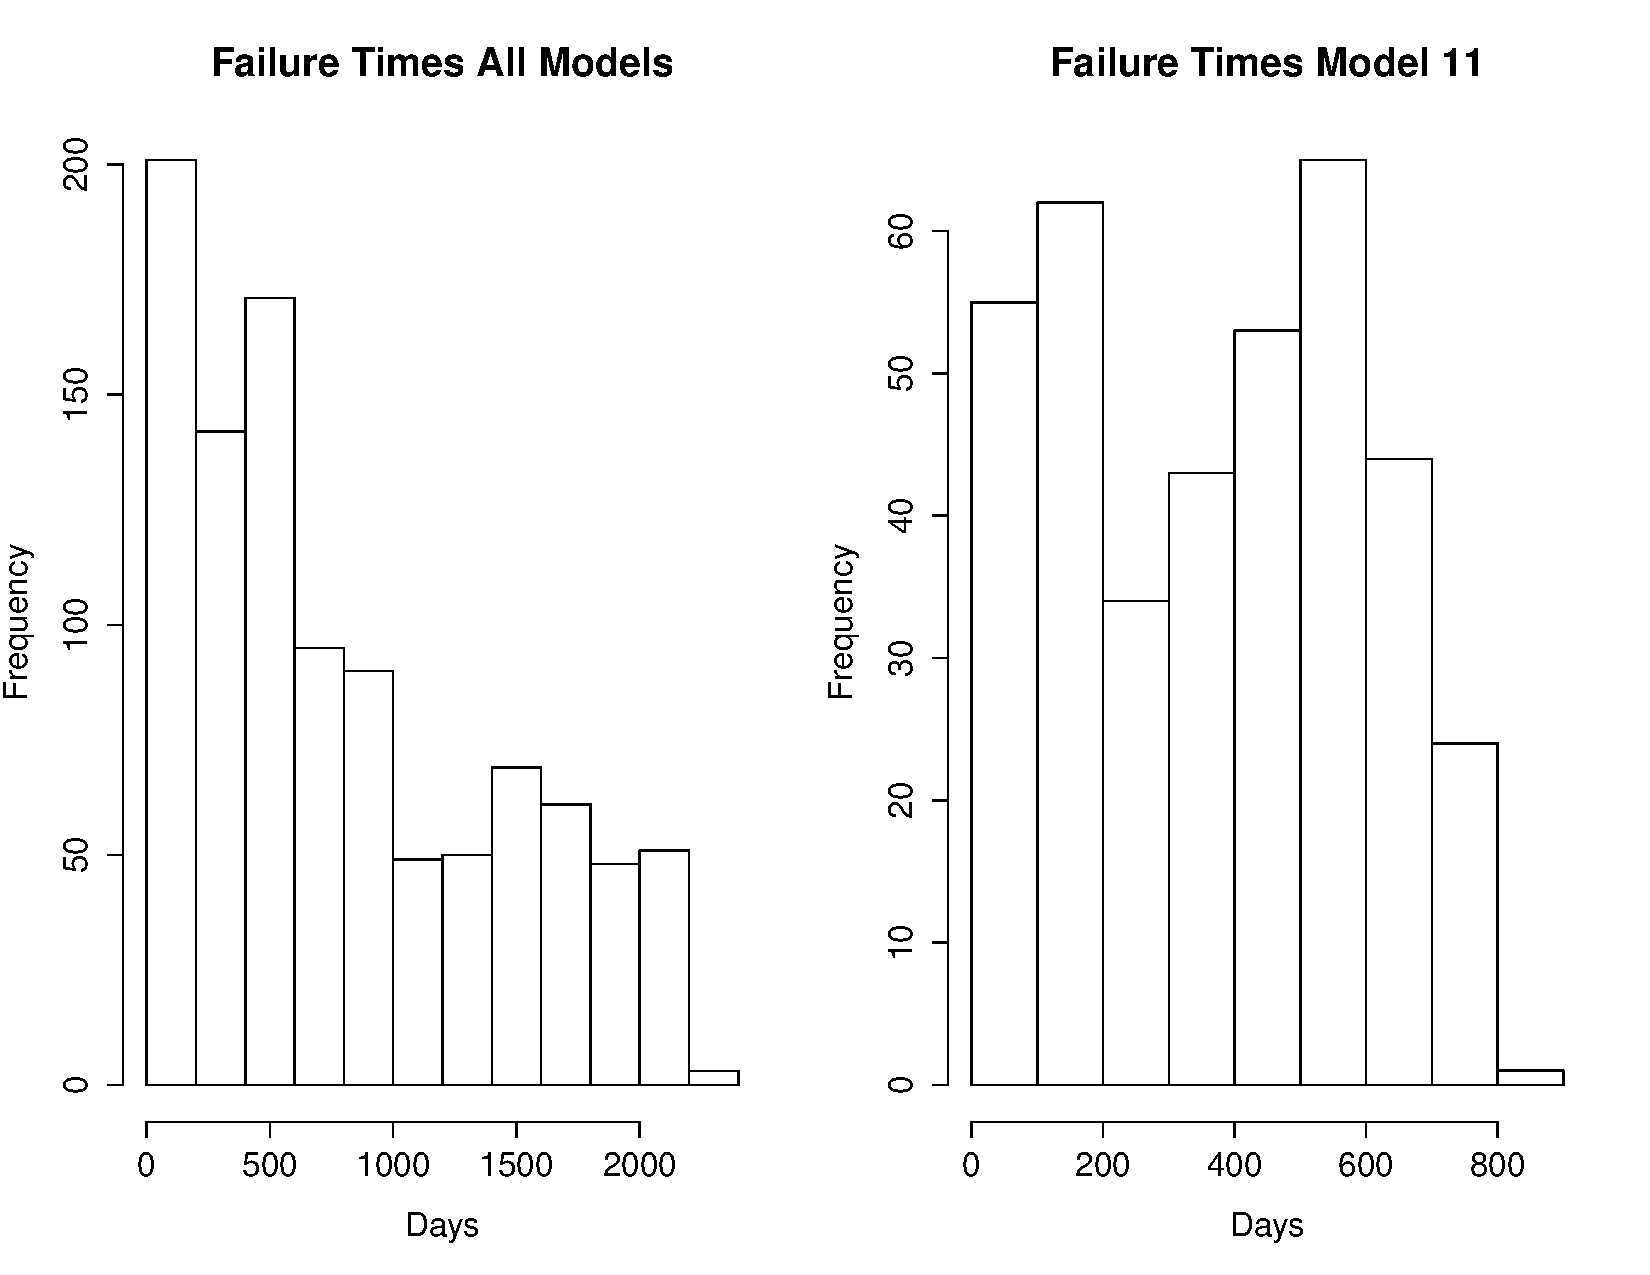
\includegraphics[height=12cm]{sumstat3.pdf}
\end{figure}
\end{document}

